\documentclass[]{elsarticle} %review=doublespace preprint=single 5p=2 column
%%% Begin My package additions %%%%%%%%%%%%%%%%%%%
\usepackage[hyphens]{url}

  \journal{Journal of Applied Ecology} % Sets Journal name


\usepackage{lineno} % add
  \linenumbers % turns line numbering on
\providecommand{\tightlist}{%
  \setlength{\itemsep}{0pt}\setlength{\parskip}{0pt}}

\usepackage{graphicx}
\usepackage{booktabs} % book-quality tables
%%%%%%%%%%%%%%%% end my additions to header

\usepackage[T1]{fontenc}
\usepackage{lmodern}
\usepackage{amssymb,amsmath}
\usepackage{ifxetex,ifluatex}
\usepackage{fixltx2e} % provides \textsubscript
% use upquote if available, for straight quotes in verbatim environments
\IfFileExists{upquote.sty}{\usepackage{upquote}}{}
\ifnum 0\ifxetex 1\fi\ifluatex 1\fi=0 % if pdftex
  \usepackage[utf8]{inputenc}
\else % if luatex or xelatex
  \usepackage{fontspec}
  \ifxetex
    \usepackage{xltxtra,xunicode}
  \fi
  \defaultfontfeatures{Mapping=tex-text,Scale=MatchLowercase}
  \newcommand{\euro}{€}
\fi
% use microtype if available
\IfFileExists{microtype.sty}{\usepackage{microtype}}{}
\usepackage[margin=1.1in]{geometry}
\bibliographystyle{elsarticle-harv}
\usepackage{longtable}
\ifxetex
  \usepackage[setpagesize=false, % page size defined by xetex
              unicode=false, % unicode breaks when used with xetex
              xetex]{hyperref}
\else
  \usepackage[unicode=true]{hyperref}
\fi
\hypersetup{breaklinks=true,
            bookmarks=true,
            pdfauthor={},
            pdftitle={Invasive mesopredator release},
            colorlinks=false,
            urlcolor=blue,
            linkcolor=magenta,
            pdfborder={0 0 0}}
\urlstyle{same}  % don't use monospace font for urls

\setcounter{secnumdepth}{5}
% Pandoc toggle for numbering sections (defaults to be off)

% Pandoc citation processing

% Pandoc header
\usepackage{setspace}\doublespacing
\usepackage{float}
\floatplacement{figure}{H}



\begin{document}
\begin{frontmatter}

  \title{Invasive mesopredator release}
    \author[UOM]{Matthew W. Rees\corref{1}}
   \ead{matt.wayne.rees@gmail.com} 
    \author[CEC]{Jack H. Pascoe}
  
    \author[UOM]{Brendan A. Wintle}
  
    \author[ARI]{Alan Robley}
  
    \author[CEC]{Mark Le Pla}
  
    \author[CEC]{Emma K. Birnbaum}
  
    \author[UOM]{Bronwyn A. Hradsky}
  
      \address[UOM]{Quantitative \& Applied Ecology Group, School of Ecosystem and Forest Science, The University of Melbourne, Parkville, VIC, Australia}
    \address[CEC]{Conservation Ecology Centre, Otway Lighthouse Rd, Cape Otway, VIC, Australia}
    \address[ARI]{Department of Environment, Land, Water and Planning, Arthur Rylah Institute for Environmental Research, Heidelberg, Australia}
      \cortext[1]{Corresponding Author}
  
  \begin{abstract}
  \begin{enumerate}
  \def\labelenumi{\arabic{enumi}.}
  \item
    Background.
  \item
    Methods.
  \item
    Results.
  \item
    \emph{Synthesis and applications.}
  \end{enumerate}
  \end{abstract}
   \begin{keyword} Camera trap; Felis catus; invasive predator; interspecific competition; mesopredator release; population density; spatial capture-recapture; spatial mark-resight; species interactions; Vulpes vulpes.\end{keyword}
 \end{frontmatter}

\parskip=12pt

\newpage

\hypertarget{introduction}{%
\section{INTRODUCTION}\label{introduction}}

Understanding species interactions is critical for effective invasive species management (Zavaleta et al., 2001). When several invasive species co-occur, management actions that suppress the dominant invasive species may inadvertently benefit subordinate invasive species (Jackson, 2015; Kuebbing \& Nuñez, 2015). Subordinate invasive species may be released from direct top-down pressure following a decline in the dominant predator or benefit indirectly from an increase in availability of shared resources (often referred to as mesopredator or competitor release - Crooks \& Soulé, 1999; Doherty \& Ritchie, 2017; Ruscoe et al., 2011). The release of a subordinate invasive species, particularly predators, can have serious negative implications for native taxa and ecosystem function (Ballari et al., 2016; Courchamp et al., 1999). However, integrated predator management is often far more costly and less feasible than single species control, and so it is important to identify when the extra cost if justified (Bode et al., 2015).

Most knowledge of predator interactions stems from unreplicated ``natural experiments'' (e.g.~range contractions - Crooks \& Soulé, 1999) or ad-hoc management interventions (e.g.~invasive species eradications - Rayner et al., 2007). However, the occurrence, nature (positive or negative, direct or indirect) and strength of species interactions can vary among species assemblages, predation risk, environmental productivity, management regimes, and other landscape contexts (Alston et al., 2019; Finke \& Denno, 2004; Hastings, 2001). Replicating management programs in an experimental framework is logistically challenging, but important for understanding these complexities, discriminating between plausible hypotheses and producing generalisable results in order to inform effective pest management (Christie et al., 2019; Glen \& Dickman, 2005; Smith et al., 2020).

Unbiased estimates of invasive predator density are important to infer native prey impacts and set meaningful control targets (Moseby et al., 2019). Controversy around the mesopredator release hypothesis partially stems from the inability to separate behavioral and numerical population processes using traditional modelling approaches (Hayward et al., 2015; Stephens et al., 2015).The suppression of an apex predator may change the behaviour and density of a mesopredator, both of which impact detection rates (Broadley et al., 2019; Rogan et al., 2019). And so--even with experimental designs--it is difficult to interpret changes in unidentified counts or presence-absence records of mesopredators in relation to apex predators. While spatially explicit capture-recapture methods have been developed to robustly estimate predator density by separating out behavioural and observational processes from population density, they have seldom been used experimentally or to investigate multispecies interactions (although, see Forsyth et al., 2019).

Predation by two invasive species, the red fox \emph{Vulpes vulpes} and feral cat \emph{Felis catus}, has played a major role in Australia's high rates of mammalian extinction (Woinarski et al.~2019). Integrated invasive predator management programs are rare. Introduced red foxes (hereafter foxes) are far more commonly controlled than feral cats, as they are more susceptible to poison-baiting, have greater direct economic impacts and fewer legal impediments to their control (McLeod \& Saunders, 2014; Reddiex et al., 2007). Nonetheless, feral cats are one of the most widespread and damaging vertebrate species (Doherty \& Ritchie, 2017; Legge et al., 2020; Medina et al., 2011). As foxes are larger-bodied (\textasciitilde2 kg difference) and have high dietary overlap with feral cats (Catling, 1988; Glen et al., 2011; Short et al., 1999), the mesopredator release hypothesis predicts that feral cat impacts will increase as fox populations are managed (Soulé et al., 1988). This is alarming because feral cats are extremely difficult to manage in open populations (Fisher et al., 2015; Lazenby et al., 2015).

Evidence that foxes suppress feral cats is inconclusive (Hunter et al., 2018). In parts of Australia where the native apex mammalian predator (the dingo \emph{Canis familiaris}) is functionally extinct and introduced foxes are the largest terrestrial mammalian predator, four studies have observed an increase in feral cat detections following fox control (Marlow et al., 2015; Risbey et al., 2000; Stobo-Wilson et al., 2020). However, two other studies in similar systems did not see any change (Molsher et al., 2017; Towerton et al., 2011). One study with spatial replication detected an increase at one site but not another (Davey et al., 2006), and one study observed a decrease in feral cat activity (Claridge et al., 2010). No previous studies have directly estimated feral cat density in response to fox control.

In this study, we experimentally investigated the role of introduced foxes in top-down suppression of feral cat density in two regions of south-eastern Australia. Foxes and feral cats are the only functional terrestrial mammalian predators in these regions, and each region included at least one area in which foxes were subject to continuous lethal poison-baiting (hereafter ``impact landscape''), and a paired area were foxes were not controlled (hereafter ``non-impact landscape''). This allowed a sharp focus on the interactions between the two invasive predators, across a gradient of apex predator (fox) occupancy and landscape productivity. Firstly, we investigated finescale associations between feral cat density and spatial fox occupancy in each region. Secondly, we tested whether fox control increased feral cat densities using traditional experimental approaches: a replicated Control-Impact design in the region with long-term fox control, and a Before-After Control-Impact Paired Series (BACIPS) design in the region with newly implemented fox control. In accordance with the mesopredator release hypothesis, we predicted that (1) feral cat density would be negatively correlated with spatial fox occupancy, and (2) fox control would increase feral cat density.
We based inference on direct estimates of feral cat density using spatially explicit mark-resight models.

\newpage

\hypertarget{materials-and-methods}{%
\section{MATERIALS AND METHODS}\label{materials-and-methods}}

\hypertarget{study-area}{%
\subsection{Study area}\label{study-area}}

We conducted our study across two regions of south-west Victoria, Australia (Fig. \ref{fig:map}). The native temperate forests in both regions are fragmented to varying degrees, primarily by livestock farming and tree plantations. Although once widespread, dingoes are now absent throughout, and a native mesopredator, the tiger quoll \emph{Dasyurus maculatus}, is long absent from the Glenelg region and recently absent in the Otway Ranges (last sighted in 2014 despite extensive camera-trapping). The terrestrial mammalian predator guild is therefore depauperate, with the introduced fox and feral cat being the primary functional mammalian terrestrial predators; birds of prey and snakes are the only other predators present.

Our study landscapes in the Glenelg region, Gunditjmara country, are primarily lowland forest (with an overstorey of \emph{Eucalyptus obliqua} and \emph{E. ovata}, a sparse midstorey and a fern-rich understorey) and heathy woodland (with an overstorey of \emph{E. baxteri s.l.} and \emph{E. willisii}, a sparse midstorey and a diverse understorey of narrow or ericoid-leaved shrubs). It has gently undulating terrain and frequently experiences prescribed burns and wildfires, creating a mosaic of fire histories and vegetation complexity. The area receives an average annual rainfall of 700 mm, with average minimum temperatures of 8.1°C and maximum of 17.6°C (\emph{Bureau of Meteorology}, 2021).

Our study landscapes in the Otway region were in the western section of the Otway Ranges, Gadubanud country. Here, the vegetation is a mosaic of shrubby wet forest and cool temperate rainforest, with an overstorey of tall eucalyptus species (primarily \emph{E. regnans}), \emph{Acacia melanoxylon} and \emph{Nothofagus cunninghamii}. The midstorey is dominated by tree ferns, \emph{Acacia verticillata}, \emph{Pomaderris aspera} and \emph{Olearia argophylla}.
The understorey predominantly comprises a dense layer of ferns and graminoids but can be relatively sparse in steep rainforest gullies. Maximum daily temperatures average 19.3°C in summer and 9.5°C in winter; annual rainfall averages 1955 mm (\emph{Bureau of Meteorology}, 2021). This region rarely experiences fire and is nearly ten times more rugged than the Glenelg region (based on the terrain ruggedness index; Riley et al., 1999, averaged within a 10 m radius of each camera-trap site).

\hypertarget{lethal-fox-control}{%
\subsection{Lethal fox control}\label{lethal-fox-control}}

Across broad sections of each region, government land managers conduct ongoing fox control for biodiversity conservation.
Manufactured poison baits (FoxOff, Animal Control Technologies, Somerton) containing 3 mg of sodium mono-fluroacetate (1080) are buried at a depth of 10 cm at 1-km intervals along accessible forest tracks and roads (Fig. \ref{fig:map}). Different road densities across the two regions therefore result in variable poison-bait densities. In the Glenelg region, fox-baiting in the impact landscapes has been ongoing since October 2005, with baits checked and replaced fortnightly (Robley et al., 2014). In the Otway region, fox-baiting commenced in the impact landscape in November 2017. Poison baits were replaced weekly for six weeks until December 2017, before changing to monthly bait replacement until July 2018. The fox control program then lapsed for approximately six months until December 2018 due to logistical constraints, when monthly bait replacement recommenced for the duration of our study (Fig. S1).

\hypertarget{study-design-and-camera-trapping}{%
\subsection{Study design and camera-trapping}\label{study-design-and-camera-trapping}}

We designed experiments around the implementation of fox-baiting in each region. We simultaneously surveyed one impact and one non-impact landscape at a time using camera-traps. Each landscape pair was chosen based on similarity in landscape context, namely vegetation groups, with the aim of maintaining spatial independence with respect to predator range movements.

In the Glenelg region, we used a replicated control-impact design to test for differences in areas that have been poison-baited for foxes for more than 13 years compared with unbaited areas. We deployed a pair of camera-trapping grids in Cobboboonee National Park (impact) and Annya State Forest (non-impact) in January -- April 2018, then moved these cameras to Mt Clay State Forest/Narrawong Flora Reserve (hereafter ``Mt Clay''; impact) and Hotspur State Forest (non-impact) in April -- June 2018 (Fig. S1). Each grid was separated by at least 8 km, a distance very unlikely to be traversed regularly by these invasive predators (Hradsky et al., 2017).

In the Otway region, we undertook a BACIPS study to assess changes related to the introduction of the fox control program. We deployed camera-trap grids in an impact -- non-impact pair of landscapes in June -- September from 2017 to 2019, in the Great Otway National Park and Otway Forest Park (Fig. S1). Our first survey occurred approximately three months before fox-baiting began. The second survey was conducted six months post-commencement of fox-baiting, however poison bait replacement lapsed at the beginning of the survey until nearly three months afterwards. Fox-baiting recommenced six months prior to the start of the final survey (Fig. S1). The impact and non-impact landscapes were at least 4.2 km apart, a distance unlikely to be traversed by these invasive predators, although possible (Hradsky et al., 2017). In this study, and a concurrent study which identified individual foxes through genetic sampling (M. Le Pla, in review), we found no evidence of either species of predator moving between these landscapes.

In each of the six survey landscapes, we deployed a grid of camera-traps (67 -- 110 cameras; mean = 94), with sites spaced on average 448 m apart (range: 194 -- 770 m; Fig. \ref{fig:map}). At each site, we deployed a single Reconyx trail camera (Reconyx, Holmen, Wisconsin) with an infrared flash and temperature-in-motion detector on a tree, facing a lure of oil-absorbing cloth doused in tuna oil (Fig. S2). More information on the camera-trapping methods is provided in Section 1.2 of the Supporting Information. Overall, we deployed 938 functional camera-traps, which operated for an average of 68 days (range: 12 -- 93 days), totalling 62,415 trap nights (Table S1) across a total study duration of five months and three years in the Glenelg and Otways regions respectively (Fig. S1).

\hypertarget{individual-feral-cat-identification}{%
\subsection{Individual feral cat identification}\label{individual-feral-cat-identification}}

We sorted the cats into five categories based on their coat type: black, mackerel tabby, classic tabby, ginger and other (cats with multiple colour blends or other distinctive coats; Fig. S3). We did not attempt to identify any black cats, even the few with white splotches on their underside, as these markings could not always be seen. Within the other four coat categories, multiple observers identified individual cats based on their unique coat patterns where possible. Detailed information on this process is provided in Section 2 of the Supporting Information.

\hypertarget{spatial-fox-occupancy}{%
\subsection{Spatial fox occupancy}\label{spatial-fox-occupancy}}

To estimate density spatially, spatial mark-resight models require covariate values for each grid cell density is estimated across, and so we could not directly use the fox data from the camera-trap sites as independent variables. We therefore used the fox presence-absence data for each camera-trap site to generate a spatially-interpolated layer of fox occupancy probability using binomial generalised additive models (Wood, 2017). We did so using the ``mgcv'' R package (version 1.3.1; Wood, 2011). We modelled fox presences and absences (response variable) across space (explanatory variable) separately for each region, with a duchon spline spatial smooth as these provide better predictions at the edge of surveyed space than other splines (Miller \& Wood, 2014). In the Otway region, we included a random intercept for each camera-trap site to account for repeat sampling and did not share spatial information across the years (using a ``by variable'' smooth with year as a factor). Differences in camera-trap deployment lengths were accounted for using a model offset. We did not use occupancy-detection models because factors which impact fox detectability on camera-traps may also impact fox detectability to feral cats - which is more important than predictive performance in this context. We predicted generalised additive models estimates into the respective spatial mark-resight habitat masks and trapfiles (detailed below).

\hypertarget{spatial-mark-resight-models-of-feral-cat-density}{%
\subsection{Spatial mark-resight models of feral cat density}\label{spatial-mark-resight-models-of-feral-cat-density}}

We used a spatial capture-recapture approach to estimate feral cat density (Borchers \& Efford, 2008). These models consider counts of detections and non-detections of individual animals at trap locations (accounting for trap-specific survey effort) to estimate the location of each individual's activity centre. These models generally assume that individuals have approximately circular home ranges and spend the majority of time in the centre of which (``activity centre''). The probability of observing an individual therefore decreases with distance from the activity centre. Two detectability parameters govern this process: g0, the probability of detecting an individual per occasion in their activity centre and sigma: a spatial scale parameter which is relative to the home range size. Multiple candidate shapes for this decline in detectability with distance from the activity centre (``detection function'') can be modelled.

Spatial capture-recapture models have been extended to consider situations where not all individuals in a population are identifiable (i.e.~marked) (Chandler \& Royle 2013). These spatial mark-resight models typically assume unmarked individuals to be a random sample of the population, sharing the same detection process as marked individuals, and so allow density to be estimated for the entire population. Spatial mark-resight models have four categories of sightings: (1) marked individuals - detections with known identities identified to the individual level at least once each session, (2) marked but unidentifiable individuals - detections of individuals with known identities, but for which the individual could not be determined in a given session (we had no detections in this category), (3) unmarked individuals - unidentified detections which definitely do not belong to the first two categories (in our study, this category comprised black cats) and (4) mark status uncertain - detections in which individuals cannot be identified and it is not clear whether the individual is of the marked or unmarked category.

We used closed population, sighting-only, spatial mark-resight to estimate feral cat density using the maximum likelihood ``secr'' R package (Efford, 2021). Detections of the ``mark status uncertain'' category cannot be handled in the ``secr'' R package, we therefore added them to the unmarked detections rather than discard them (Moseby et al., 2020). We condensed detection histories of each mark category to a binary presence-absence record per each camera-trap for a 24-hour length duration (``occasion''), beginning at midday. We ran separate models for each region and treated each camera-trap grid deployment as a ``session''. We created a 4000 metre buffer zone around each camera-trap location to estimate feral cat density across, with a grid cell resolution of 200 metres. These habitat mask specifications were based on initial models and our knowledge of feral cats in these area - ensuring density is estimated over a large enough area to encompass the activity centres of all feral cats exposed to our camera-traps, at a fine enough scale to minimise bias in density estimates. We tested the half-normal and exponential detection functions in each region, carrying forward the function with the lowest Akaike's Information Criterion score adjusted for small sample size (AICc) for all subsequent model fitting (Burnham \& Anderson, 2004).

For each of the two regions, we ran three sets of models where we: (1) chose ``base model'' covariates to carry through into subsequent model sets, (2) tested fine-scale associations between spatial fox occupancy and feral cat density, and (3) experimentally evaluated the effect of fox control on feral cat density. We assessed the relative performance of models in each set using AICc score, with models within 2 delta AICc of the top-ranked model considered strongly supported compared to the other candidate models (Burnham \& Anderson, 2004). We expected that foxes would impact both detectability parameters for feral cats concurrently, and so, always specified g0 and sigma consistently in relation to foxes or fox control (Efford \& Mowat, 2014).

Feral cat detectability may have decreased over each survey duration due to lure scent fading, and density may differ across vegetation types. While we chose landscape pairs based on the similarity of ecological vegetation class groups (DELWP, 2020), there were small differences in the relative proportion of each group across landscapes. To account for this, we first condensed vegetation groups into three categories for each region: cleared land, heathy woodlands, lowland forests (Glenelg region only) and wet forests (Otways region only). Detailed information on this process is provided in Section 6 of the Supporting Information. We included vegetation type as a habitat mask covariate. Camera-traps were lured with tuna oil scent, which likely faded over the survey duration and potentially reduced feral cat detectability (Rees et al., 2019). To account for this, we fit a model where g0 had a linear trend over over the survey duration for each camera-trap. We included year as a density covariate in the Otway region models to account for repeat sampling. We compared these models to a ``null model'' where feral cat density and detectability was constant. We carried these covariates through to all subsequent model fits if their respective model had an AICc score which was lower than the null model by more than two.

To test direct associations between feral cats and foxes, we used the spatial fox occupancy estimates (detailed in the previous section) as an explanatory variable. We fit three models in each region; (1) where fox occupancy only affected feral cat density, (2) where fox occupancy only affected feral cat detectability (both parameters), and (3) fox occupancy affected both the density and detectability of feral cats. We included year as a density covariate in the Otway region models to account for repeat sampling. We assessed these three models relative to a respective null model which did not include the fox occupancy covariate. We considered support for an association between feral cats and foxes if any of these models had an AICc score which was lower than the null model by more than two.

To investigate fox-baiting effects, we compared the difference in feral cat density between paired non-impact and impact landscapes. We estimated density separately for each landscape and considered statistical evidence for a difference between paired landscapes if 95\% confidence intervals of the coefficient estimates of difference did not overlap zero. We used AICc scores to choose between different specifications of the detectability parameters: (1) constant, (2) an effect of fox-baiting (but with separate effects in each spatial or temporal replicate), (3) an effect of pair in the Glenelg region (due seasonal difference) or an effect of year in the Otway region, (4) the combination of fox-baiting and pair/year effects--only presenting the top-ranked model.

\newpage

\begin{figure}
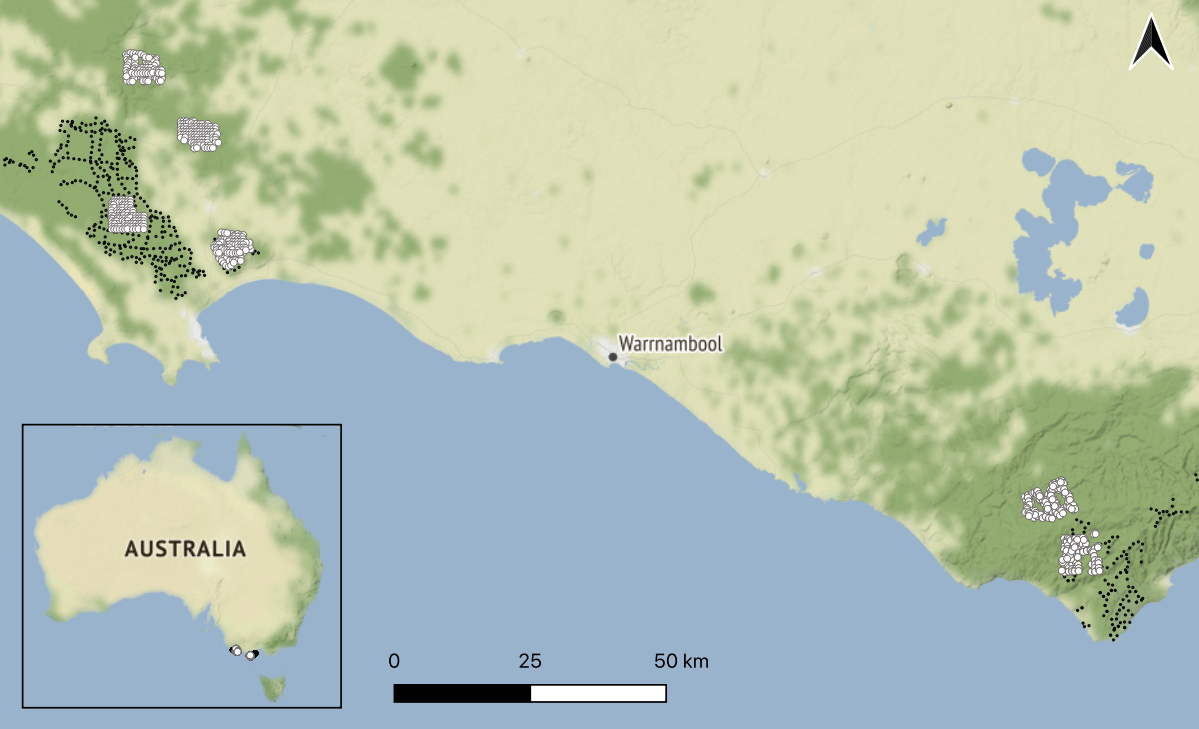
\includegraphics[width=1\linewidth]{figs/fig1} \caption{Locations of our six study landscapes in south-west Victoria, Australia. The grids of camera-traps are denoted by white dots, the locations of fox poison-bait stations are denoted by smaller black dots. The Glenelg region is to the west and Otway region to the east. Native vegetation is indicated by dark green, with hill shading. Map tiles by Stamen Design, under CC BY 3.0, map data by OpenStreetMap, under CC BY SA.}\label{fig:map}
\end{figure}

\newpage

\hypertarget{results}{%
\section{RESULTS}\label{results}}

\hypertarget{fox-occupancy}{%
\subsection{Fox occupancy}\label{fox-occupancy}}

In the Glenelg region, foxes were detected on 0.55 and 0.26 of camera-trap sites in the non-impact and impact landscapes for the first replicate (Annya and Cobboboonee, respectively). For the second landscape pair replicate, foxes were detected at 0.48 and 0.35 of the camera-trap sites (Hotspur and Mt Clay, respectively). In the non-impact landscape of the Otway Ranges, naive fox occupancy rates increased from 0.13 in 2017, to 0.27 in 2018, to 0.43 in 2019. Foxes were detected at 0.36 of sites in the Otway impact landscape prior to poison-baiting in 2017, decreasing to 0.27 in 2018 (where fox-baiting occurred prior to, but lapsed during this survey), and further to 0.17 in 2019 (where fox-baiting occurred during the survey and had been for six months prior).

The generalised additive models of fox occupancy (which accounted for the different camera-trap survey durations) produced occupancy estimates in each region, which, when averaged at the landscape level (i.e.~the mean cell value for each landscape in Fig. \ref{fig:foxplot}), were largely consistent with the unadjusted naive occupancy rates. In the Glenelg region, mean fox occupancy was 0.51 (SE 0.13) and 0.34 (SE 0.12) for the first non-impact and impact replicate, with a mean estimate of 0.56 (SE 0.13) and 0.51 (SE 0.14) for the second replicate pair. In the Otway region, mean fox occupancy in the non-impact landscape changed from 0.18, 0.23, 0.36 in 2017, 2018 and 2019 (respective SEs: 0.07, 0.03, 0.11), whereas mean fox occupancy in the impact landscape changed from 0.31, 0.23, 0.18 in 2017, 2018 and 2019 (respective SEs: 0.09, 0.03, 0.08). There was higher fine-scale spatial variation in fox occupancy within the Glenelg region compared to the Otway region (Fig. \ref{fig:foxplot}). In fact, a completely smooth relationship (i.e.~no spatial variation with space was predicted for the 2018 survey in the Otway region (Fig. \ref{fig:foxplot}). The Glenelg region generalised additive model had an adjusted R-squared value of 0.142 and explained 14.8\% deviance, whereas the Otway region model had an R-squared value of 0.24 and explained 27.8\% deviance. Model summaries and spatial standard error estimates are presented in Section 5 of the Supporting Information.

\hypertarget{feral-cats-in-the-glenelg-region}{%
\subsection{Feral cats in the Glenelg region}\label{feral-cats-in-the-glenelg-region}}

In the Glenelg region, we recorded 222 feral cat detections from 26,792 camera-trap nights (Table S1). Sixty-five percent of detections were feral cats with unique natural markings; the remainder were black feral cats. We identified 85\% of marked feral cats to the individual level; a total of 40 cats (9 -- 13 individuals per grid). The exponential detector function was strongly supported over the half-normal (Table S2). There was no support for a linear time trend on g0, nor for an impact of vegetation type on feral cat density (Table S3).

Feral cat density was negatively associated with spatial fox occupancy (coefficient -1.59; standard error 0.71; Fig. \ref{fig:dcor}). This model was well-supported; models which included an impact of fox occupancy on detectability parameters performed worse than the null model based on AICc scores (Table S3).

When we estimated feral cat density separately for each landscape, there was statistical evidence (i.e., 95\% confidence intervals of the parameter estimates did not overlap zero) that feral cat density was higher in the first impact landscape than its associated non-impact landscapes
for the first replicate, but no difference for the second replicate (Fig. \ref{fig:diffg}). The top-model in this set also had detectability as constant.

\hypertarget{feral-cats-in-the-otway-region}{%
\subsection{Feral cats in the Otway region}\label{feral-cats-in-the-otway-region}}

In the Otway region, we recorded 1022 feral cat detections from 35,623 camera-trap nights (Table S1). Sixty-one percent of detections were of feral cats with unique natural markings and we identified 86\% of these, a total of 98 cats (20 -- 30 per grid). The exponential detector function was strongly supported over the half-normal (Table S2). There was no support for a linear time trend on g0, nor for an impact of vegetation type on feral cat density (Table S3).

Spatial fox occupancy was negatively correlated with feral cat density (coefficient -1.57; standard error 0.80; Fig. \ref{fig:dcor}) and also impacted feral cat detectability (Fig. \ref{fig:detcor}). Where fox occupancy was higher, feral cats were less detectable in their activity centres (i.e.~negative association with g0; coefficient -3.52; standard error 1.17; Fig. \ref{fig:detcor}A) and ranged further (i.e.~positive association with sigma; coefficient 1.54; standard error 0.50; Fig. \ref{fig:detcor}B).

There was no statistical evidence that feral cat density differed between impact and non-impact sites in any of the three years surveyed (Fig. \ref{fig:diffo}A). The coefficient estimate of difference changed from a negative direction in 2017 and 2018 (i.e.~feral cat density was lower in the impact site than the non-impact site) to a positive direction in 2019 (when fox-baiting occurred throughout the survey duration), however 95\% confidence intervals of the parameter estimates overlapped overlap zero (Fig. \ref{fig:diffo}A). There was strong evidence (based on AICc scores) that feral cat detectability differed across the three years, and in response to the fox-baiting (Table S5). In the non-impact site, there appeared to be a decline in feral cat density over the three years surveyed (although we did not explicitly test the statistical significance of this; Fig. \ref{fig:diffo}B).

\newpage

\begin{figure}
\includegraphics[width=1\linewidth]{figs/fig2_600dpi} \caption{Fox probability of occupancy derived from generalised additive models within each impact (I) and associated non-impact (NI) landscape in the Glenelg (A) and Otways (B) regions. Estimates were used as predictor variables in the feral cat spatial mark-resight models.}\label{fig:foxplot}
\end{figure}

\newpage

\begin{figure}
\includegraphics[width=1\linewidth]{figs/foxD_600dpi} \caption{Feral cat density declined with increasing probability of fox occupancy in both the Glenelg and Otway regions. Shaded areas indicate 95\% confidence intervals.}\label{fig:dcor}
\end{figure}

\newpage

\begin{figure}
\includegraphics[width=1\linewidth]{figs/foxDet_otways_600dpi} \caption{In the Otway Ranges, the probability of detecting a feral cat in its activity centre per 24-hour occasion (g0) increased with the probability of fox occupancy (B), while sigma (which is related to home range size) increased (C). Shaded areas indicate 95\% confidence intervals.}\label{fig:detcor}
\end{figure}

\newpage

\begin{figure}
\includegraphics[width=1\linewidth]{figs/glenelg_estimates_600dpi} \caption{Estimates of difference between feral cat density in impact and non-impact landscapes (A) and predicted density estimates (B) in the Glenelg region, Australia. There was statistical evidence (i.e., 95\% confidence intervals of the parameter estimates did not overlap zero) that feral cat density was higher in the landscape with more than 13 years of fox-baiting (impact) than landscapes without fox-baiting (non-impact) for the first replicate pair, but not for the second replicate pair. Error bars represent 95\% confidence intervals.}\label{fig:diffg}
\end{figure}

\newpage

\begin{figure}
\includegraphics[width=1\linewidth]{figs/otways_estimates_600dpi} \caption{Estimates of difference between impact and non-impact landscapes (A) and predicted density estimates (B) in the Otway region, Australia. There was not statistical evidence (95\% confidence intervals of the parameter estimates overlapped zero) that feral cat density differed between impact and non-impact landscapes in each year surveyed). In 2017, surveys were conducted approximately two months before fox control commenced in the impact landscape (red). Error bars represent 95\% confidence intervals.}\label{fig:diffo}
\end{figure}

\newpage

\hypertarget{discussion}{%
\section{DISCUSSION}\label{discussion}}

Feral cat density was highest where fox occupancy was lowest across both regions (supporting hypothesis 1), but feral cat density did not consistently increase following lethal fox control (mixed support for hypothesis 2). We expect this to be partly due to variable effectiveness of fox control across space and time, and partly due to our short sampling period in the Otway region post-baiting - there was likely not enough time for a numerical changes to occur at an effect size we could reliably detect. However we did detect behavioural changes in the Otway Ranges. Our study highlights the nuance involved in detecting mesopredator release, demonstrating how correlative and experimental approaches provide complementary lines of evidence and the importance of distinguishing behavioural and numerical responses.

Feral cat density in the Glenelg region was consistent across three out of the four landscapes surveyed. This is unsurprising given that (1) feral cat density was negatively correlated with fox occupancy, and (2) landscape-wide fox occupancy estimates varied by less than 10\% in these three landscapes. In contrast, fox occupancy was at least 31\% lower on average in Cobboboonee, with cat density at least 67\% higher. Relative to this landscape, Mt Clay has a high fox occupancy landscape-average because the camera-trap grid was nearly entirely surrounded by unbaited farmland (whereas the Cobboboonee habitat mask mostly consisted of fox-baited forest; Fig. S11). Hradsky et al. (2019) predicted a 1 km poison-baited buffer zone in the surrounding farmland around Mt Clay could reduce fox density by 58\%, which our observations support - fox occupancy was low in the forest interior (Fig. \ref{fig:foxplot}A). While experimental studies are fundamental to testing the mesopredator release theory, direct measurements of apex predators are also necessary to understand mesopredator responses. The highly variable outcomes of lethal apex predator control adds an extra layer of confusion around predator interactions for studies that use impact and non-impact as a proxy for apex predator abundance and distribution (e.g.~Hunter et al., 2018).

Prior to fox control, landscape-average fox occupancy in the Otway Ranges was lower than landscapes subject to 13 years of continuous fox-baiting in the Glenelg region. Dexter \& Murray (2009) hypothesised that fox control can decrease fox abundance substantially beyond baited landscapes, however, fox occupancy doubled over the three years we surveyed in Otway Ranges non-impact site (which is proximal to the impact site). We are not sure why fox occupancy increased here (or whether it is was related to the impact site). Regardless, feral cat density had the opposite response to foxes and declined in the non-impact site over the three years (Fig. \ref{fig:diffo}B). In the impact site, average fox occupancy decreased by 42\% and while feral cat density did not decrease, the rate of decline stopped in 2019 and for the first time, density was estimated to be higher in the impact landscape. Indeed, like the Glenelg region, we saw evidence that feral cat density was negatively correlated with fox occupancy. However, there was no statistical evidence that feral cat density differed between the impact and non-impact landscapes.

Either fox-baiting did not directly effect feral cat density in the Otway Ranges within this time period (despite the negative fox-cat correlation), or the effect was weaker than we had power to detect. Despite high feral cat density, confidence intervals were large due to the high proportion of unmarked cats, and complex detectability covariates. This severely limited our ability to detect small changes in feral cat density directly due to fox control. Additionally, we would expect weaker fox-baiting effects in the Otway Ranges because fox occupancy was already low (less top-pressure on feral cats) and fox control was less intensive (poison-bait replacement occurred twice as infrequent and there was a six month pause in 2018) than the Glenelg region. Further, we only surveyed 1.5 years following the commencement of fox control. We would also expect a lagged response of feral cat density to fox control because (1) foxes are more likely to reduce feral cat reproductive and recruitment rates, rather than directly killing adult feral cats, and (2) this explains patterns in prey populations following fox control. Native prey populations often ``erupt'' after fox control commences, before subsequently crashing (Duncan et al., 2020). These population prey population crashes could be due to prey overshooting carrying capacity following relaxed top-down pressure, although, that doesn't alone explain overall declines and extinctions in prey following long-term fox control (refs). Regardless, we saw a negative correlation between foxes and feral cats, which demonstrates that a mesopredator release due to fox control is possible in the Otway Ranges. Our study provides a strong foundation to compare future changes in predator and prey populations against.

Where fox occupancy was higher in the Otway Ranges, feral cats were less detectable in their activity centres and ranged further (Fig. S11). Similar responses have been seen elsewhere, such as foxes in response to coyote Canis latrans presence (Lombardi et al.~2017). Our result suggests that feral cats are avoiding foxes, though the specific behaviour of avoidance should be tested. Animals also tend to range further when their density is lower (Broadley et al.~2019). Apex predators may therefore alter mesopredator movement behaviour directly due to fear, or indirectly by supressing their density, which in turn affects movement behaviour. These two processes need to be considered relying solely on unmarked detections---mesopredator release has the potential to increase (perceived) spatial overlap between the predator species for certain study designs (Efford \& Dawson 2012; Neilson et al.~2018; Broadley et al.~2019).

\newpage

\hypertarget{conclusions}{%
\section{CONCLUSIONS}\label{conclusions}}

\newpage

\hypertarget{acknowledgements}{%
\section{ACKNOWLEDGEMENTS}\label{acknowledgements}}

We acknowledge and pay respect to the Gadubanud and Gunditjmara people on whose traditional lands this study took place. Surveys were conducted under University of Melbourne Animal Ethics Committee approval 1714119 and Victorian Government Department of Environment, Land Water and Planning Research Permit 10008273. This experiment was a collaborative effort between the Glenelg Ark (Department of Environment, Land Water and Planning) and Otway Ark (Parks Victoria) working groups.
We are extremely grateful to our field assistants: Shauni Omond, Shayne Neal, Asitha Samarawickrama, Shelley Thompson, Erin Harris, Hannah Killian, Lani Watson, Mark Dorman, Jack Davis, Carl Roffey, Bruce Edley, Larissa Oliveira Gonçalves, Ben Lake, Chantelle Geissler, Aviya Naccarella, Emily Gronow, Harley England, David Pitts, Annie Hobby, Louise Falls, Thomas McKinnon, Jimmy Downie, Marney Hradsky, Stephanie Samson, Robin Sinclair, Asmaa Alhusainan, Kelly Forrester, Tammana Wadawani, Emily McColl-Gausden, Emily Gregg, Hannah Edwards, Adam Beck, Vishnu Memnon, Sandy Lu, Pia Lentini, Nick Golding, Emily McColl-Gausden, Nina Page, Maggie Campbell-Jones, Kyle Quinn and Jack Dickson. This manuscript was improved by comments from William Geary. Our study was generously supported by the Conservation Ecology Centre, the Victorian Government Department of Environment, Land Water and Planning, Arthur Rylah Institute for Environmental Research, Parks Victoria and the Australian Government's National Environmental Science Program through the Threatened Species Recovery Hub, and ARC Linkage Project LP170101134. MR also receives support from an Australian Government Research Training Program Scholarship.

\hypertarget{authors-contributions}{%
\section{AUTHORS' CONTRIBUTIONS}\label{authors-contributions}}

M.W.R, B.H, J.H.P, B.A.W and A.R conceived the ideas and designed methodology; M.W.R, J.H.P, M.LP, E.K.B and B.H collected the data; M.W.R analysed the data; M.W.R led the writing of the manuscript. All authors contributed critically to the drafts and gave final approval for publication.

\hypertarget{open-research}{%
\section{OPEN RESEARCH}\label{open-research}}

Raw data and code are on Github link xx.\\
Data will be deposited on the Dryad Digital Repository after acceptance.

\newpage

\hypertarget{references}{%
\section*{REFERENCES}\label{references}}
\addcontentsline{toc}{section}{REFERENCES}

\hypertarget{refs}{}
\leavevmode\hypertarget{ref-alston2019}{}%
Alston, J., Maitland, B., Brito, B., Esmaeili, S., Ford, A., Hays, B., Jesmer, B., Molina, F., \& Goheen, J. (2019). Reciprocity in restoration ecology: When might large carnivore reintroduction restore ecosystems? \emph{Biological Conservation}, \emph{234}, 82--89.

\leavevmode\hypertarget{ref-ballari2016}{}%
Ballari, S. A., Kuebbing, S. E., \& Nuñez, M. A. (2016). Potential problems of removing one invasive species at a time: A meta-analysis of the interactions between invasive vertebrates and unexpected effects of removal programs. \emph{PeerJ}, \emph{4}, e2029.

\leavevmode\hypertarget{ref-bode2015}{}%
Bode, M., Baker, C. M., \& Plein, M. (2015). Eradicating down the food chain: Optimal multispecies eradication schedules for a commonly encountered invaded island ecosystem. \emph{Journal of Applied Ecology}, \emph{52}(3), 571--579.

\leavevmode\hypertarget{ref-borchers2008}{}%
Borchers, D. L., \& Efford, M. G. (2008). Spatially explicit maximum likelihood methods for capture--recapture studies. \emph{Biometrics}, \emph{64}(2), 377--385.

\leavevmode\hypertarget{ref-broadley2019}{}%
Broadley, K., Burton, A. C., Avgar, T., \& Boutin, S. (2019). Density-dependent space use affects interpretation of camera trap detection rates. \emph{Ecology and Evolution}, \emph{9}(24), 14031--14041.

\leavevmode\hypertarget{ref-BOM2021}{}%
\emph{Bureau of meteorology}. (2021). Climate Data Online URL; (accessed May 2021). \url{http://www.bom.gov.au/climate/data/}

\leavevmode\hypertarget{ref-burnham2004}{}%
Burnham, K. P., \& Anderson, D. R. (2004). Multimodel inference: Understanding aic and bic in model selection. \emph{Sociological Methods \& Research}, \emph{33}(2), 261--304.

\leavevmode\hypertarget{ref-catling1988}{}%
Catling, P. (1988). Similarities and contrasts in the diets of foxes, vulpes vulpes, and cats, felis catus, relative to fluctuating prey populations and drought. \emph{Wildlife Research}, \emph{15}(3), 307--317.

\leavevmode\hypertarget{ref-christie2019}{}%
Christie, A. P., Amano, T., Martin, P. A., Shackelford, G. E., Simmons, B. I., \& Sutherland, W. J. (2019). Simple study designs in ecology produce inaccurate estimates of biodiversity responses. \emph{Journal of Applied Ecology}, \emph{56}(12), 2742--2754.

\leavevmode\hypertarget{ref-claridge2010}{}%
Claridge, A. W., Cunningham, R. B., Catling, P. C., \& Reid, A. M. (2010). Trends in the activity levels of forest-dwelling vertebrate fauna against a background of intensive baiting for foxes. \emph{Forest Ecology and Management}, \emph{260}(5), 822--832.

\leavevmode\hypertarget{ref-courchamp1999}{}%
Courchamp, F., Langlais, M., \& Sugihara, G. (1999). Cats protecting birds: Modelling the mesopredator release effect. \emph{Journal of Animal Ecology}, \emph{68}(2), 282--292.

\leavevmode\hypertarget{ref-crooks1999}{}%
Crooks, K. R., \& Soulé, M. E. (1999). Mesopredator release and avifaunal extinctions in a fragmented system. \emph{Nature}, \emph{400}(6744), 563--566.

\leavevmode\hypertarget{ref-davey2006}{}%
Davey, C., Sinclair, A., Pech, R. P., Arthur, A. D., Krebs, C. J., Newsome, A., Hik, D., Molsher, R., \& Allcock, K. (2006). Do exotic vertebrates structure the biota of australia? An experimental test in new south wales. \emph{Ecosystems}, \emph{9}(6), 992--1008.

\leavevmode\hypertarget{ref-delwp2020}{}%
DELWP. (2020). \emph{Bioregions and evc benchmarks}. Victorian Government Department of Environment, Land, Water; Planning, Melbourne. Accessed June 2021). \url{https://www.environment.vic.gov.au/biodiversity/bioregions-and-evc-benchmarks}

\leavevmode\hypertarget{ref-dexter2009impact}{}%
Dexter, N., \& Murray, A. (2009). The impact of fox control on the relative abundance of forest mammals in east gippsland, victoria. \emph{Wildlife Research}, \emph{36}(3), 252--261.

\leavevmode\hypertarget{ref-doherty2017}{}%
Doherty, T. S., \& Ritchie, E. G. (2017). Stop jumping the gun: A call for evidence-based invasive predator management. \emph{Conservation Letters}, \emph{10}(1), 15--22.

\leavevmode\hypertarget{ref-duncan2020eruptive}{}%
Duncan, R. P., Dexter, N., Wayne, A., \& Hone, J. (2020). Eruptive dynamics are common in managed mammal populations. \emph{Ecology}, \emph{101}(12), e03175.

\leavevmode\hypertarget{ref-efford2021secr}{}%
Efford, M. G. (2021). \emph{Secr: Spatially explicit capture-recapture models. R package version 4.4.4}. (accessed June 2021). \url{http://CRAN.R-project.org/package=secr}

\leavevmode\hypertarget{ref-finke2004}{}%
Finke, D. L., \& Denno, R. F. (2004). Predator diversity dampens trophic cascades. \emph{Nature}, \emph{429}(6990), 407--410.

\leavevmode\hypertarget{ref-fisher2015}{}%
Fisher, P., Algar, D., Murphy, E., Johnston, M., \& Eason, C. (2015). How does cat behaviour influence the development and implementation of monitoring techniques and lethal control methods for feral cats? \emph{Applied Animal Behaviour Science}, \emph{173}, 88--96.

\leavevmode\hypertarget{ref-forsyth2019}{}%
Forsyth, D. M., Ramsey, D. S., \& Woodford, L. P. (2019). Estimating abundances, densities, and interspecific associations in a carnivore community. \emph{The Journal of Wildlife Management}, \emph{83}(5), 1090--1102.

\leavevmode\hypertarget{ref-glen2011}{}%
Glen, A., Pennay, M., Dickman, C., Wintle, B., \& Firestone, K. (2011). Diets of sympatric native and introduced carnivores in the barrington tops, eastern australia. \emph{Austral Ecology}, \emph{36}(3), 290--296.

\leavevmode\hypertarget{ref-glen2005}{}%
Glen, A. S., \& Dickman, C. R. (2005). Complex interactions among mammalian carnivores in australia, and their implications for wildlife management. \emph{Biological Reviews}, \emph{80}(3), 387--401.

\leavevmode\hypertarget{ref-hastings2001}{}%
Hastings, A. (2001). Transient dynamics and persistence of ecological systems. \emph{Ecology Letters}, \emph{4}(3), 215--220.

\leavevmode\hypertarget{ref-hayward2015}{}%
Hayward, M. W., Boitani, L., Burrows, N. D., Funston, P. J., Karanth, K. U., MacKenzie, D. I., Pollock, K. H., \& Yarnell, R. W. (2015). Ecologists need robust survey designs, sampling and analytical methods. \emph{Journal of Applied Ecology}, \emph{52}(2), 286--290.

\leavevmode\hypertarget{ref-hradsky2019foxnet}{}%
Hradsky, B. A., Kelly, L. T., Robley, A., \& Wintle, B. A. (2019). FoxNet: An individual-based model framework to support management of an invasive predator, the red fox. \emph{Journal of Applied Ecology}, \emph{56}(6), 1460--1470.

\leavevmode\hypertarget{ref-hradsky2017human}{}%
Hradsky, B. A., Robley, A., Alexander, R., Ritchie, E. G., York, A., \& Di Stefano, J. (2017). Human-modified habitats facilitate forest-dwelling populations of an invasive predator, vulpes vulpes. \emph{Scientific Reports}, \emph{7}(1), 1--12.

\leavevmode\hypertarget{ref-hunter2018}{}%
Hunter, D. O., Lagisz, M., Leo, V., Nakagawa, S., \& Letnic, M. (2018). Not all predators are equal: A continent-scale analysis of the effects of predator control on australian mammals. \emph{Mammal Review}, \emph{48}(2), 108--122.

\leavevmode\hypertarget{ref-jackson2015}{}%
Jackson, M. C. (2015). Interactions among multiple invasive animals. \emph{Ecology}, \emph{96}(8), 2035--2041.

\leavevmode\hypertarget{ref-kuebbing2015}{}%
Kuebbing, S. E., \& Nuñez, M. A. (2015). Negative, neutral, and positive interactions among nonnative plants: Patterns, processes, and management implications. \emph{Global Change Biology}, \emph{21}(2), 926--934.

\leavevmode\hypertarget{ref-lazenby2015}{}%
Lazenby, B. T., Mooney, N. J., \& Dickman, C. R. (2015). Effects of low-level culling of feral cats in open populations: A case study from the forests of southern tasmania. \emph{Wildlife Research}, \emph{41}(5), 407--420.

\leavevmode\hypertarget{ref-legge2020}{}%
Legge, S., Taggart, P. L., Dickman, C. R., Read, J. L., \& Woinarski, J. C. (2020). \emph{Wildlife Research}, \emph{47}(8), 731--746.

\leavevmode\hypertarget{ref-marlow2015}{}%
Marlow, N. J., Thomas, N. D., Williams, A. A., Macmahon, B., Lawson, J., Hitchen, Y., Angus, J., \& Berry, O. (2015). Cats (felis catus) are more abundant and are the dominant predator of woylies (bettongia penicillata) after sustained fox (vulpes vulpes) control. \emph{Australian Journal of Zoology}, \emph{63}(1), 18--27.

\leavevmode\hypertarget{ref-mcleod2014}{}%
McLeod, S. R., \& Saunders, G. (2014). Fertility control is much less effective than lethal baiting for controlling foxes. \emph{Ecological Modelling}, \emph{273}, 1--10.

\leavevmode\hypertarget{ref-medina2011}{}%
Medina, F. M., Bonnaud, E., Vidal, E., Tershy, B. R., Zavaleta, E. S., Josh Donlan, C., Keitt, B. S., Le Corre, M., Horwath, S. V., \& Nogales, M. (2011). A global review of the impacts of invasive cats on island endangered vertebrates. \emph{Global Change Biology}, \emph{17}(11), 3503--3510.

\leavevmode\hypertarget{ref-miller2014}{}%
Miller, D. L., \& Wood, S. N. (2014). Finite area smoothing with generalized distance splines. \emph{Environmental and Ecological Statistics}, \emph{21}(4), 715--731.

\leavevmode\hypertarget{ref-molsher2017}{}%
Molsher, R., Newsome, A. E., Newsome, T. M., \& Dickman, C. R. (2017). Mesopredator management: Effects of red fox control on the abundance, diet and use of space by feral cats. \emph{PLoS One}, \emph{12}(1), e0168460.

\leavevmode\hypertarget{ref-moseby2019}{}%
Moseby, K. E., Letnic, M., Blumstein, D. T., \& West, R. (2019). Understanding predator densities for successful co-existence of alien predators and threatened prey. \emph{Austral Ecology}, \emph{44}(3), 409--419.

\leavevmode\hypertarget{ref-moseby2020effectiveness}{}%
Moseby, K., McGregor, H., \& Read, J. (2020). Effectiveness of the felixer grooming trap for the control of feral cats: A field trial in arid south australia. \emph{Wildlife Research}, \emph{47}(8), 599--609.

\leavevmode\hypertarget{ref-rayner2007}{}%
Rayner, M. J., Hauber, M. E., Imber, M. J., Stamp, R. K., \& Clout, M. N. (2007). Spatial heterogeneity of mesopredator release within an oceanic island system. \emph{Proceedings of the National Academy of Sciences}, \emph{104}(52), 20862--20865.

\leavevmode\hypertarget{ref-reddiex2007}{}%
Reddiex, B., Forsyth, D. M., McDonald-Madden, E., Einoder, L. D., Griffioen, P. A., Chick, R. R., \& Robley, A. J. (2007). Control of pest mammals for biodiversity protection in australia. I. Patterns of control and monitoring. \emph{Wildlife Research}, \emph{33}(8), 691--709.

\leavevmode\hypertarget{ref-rees2019}{}%
Rees, M., Pascoe, J., Wintle, B., Le Pla, M., Birnbaum, E., \& Hradsky, B. (2019). Unexpectedly high densities of feral cats in a rugged temperate forest. \emph{Biological Conservation}, \emph{239}, 108287.

\leavevmode\hypertarget{ref-riley1999}{}%
Riley, S. J., DeGloria, S. D., \& Elliot, R. (1999). Index that quantifies topographic heterogeneity. \emph{Intermountain Journal of Sciences}, \emph{5}(1-4), 23--27.

\leavevmode\hypertarget{ref-risbey2000}{}%
Risbey, D. A., Calver, M. C., Short, J., Bradley, J. S., \& Wright, I. W. (2000). The impact of cats and foxes on the small vertebrate fauna of heirisson prong, western australia. II. A field experiment. \emph{Wildlife Research}, \emph{27}(3), 223--235.

\leavevmode\hypertarget{ref-robley2014}{}%
Robley, A., Gormley, A. M., Forsyth, D. M., \& Triggs, B. (2014). Long-term and large-scale control of the introduced red fox increases native mammal occupancy in australian forests. \emph{Biological Conservation}, \emph{180}, 262--269.

\leavevmode\hypertarget{ref-rogan2019}{}%
Rogan, M. S., Balme, G. A., Distiller, G., Pitman, R. T., Broadfield, J., Mann, G. K., Whittington-Jones, G. M., Thomas, L. H., \& O'Riain, M. J. (2019). The influence of movement on the occupancy--density relationship at small spatial scales. \emph{Ecosphere}, \emph{10}(8), e02807.

\leavevmode\hypertarget{ref-ruscoe2011}{}%
Ruscoe, W. A., Ramsey, D. S., Pech, R. P., Sweetapple, P. J., Yockney, I., Barron, M. C., Perry, M., Nugent, G., Carran, R., Warne, R., \& others. (2011). Unexpected consequences of control: Competitive vs. Predator release in a four-species assemblage of invasive mammals. \emph{Ecology Letters}, \emph{14}(10), 1035--1042.

\leavevmode\hypertarget{ref-short1999}{}%
Short, J., Calver, M. C., \& Risbey, D. A. (1999). The impact of cats and foxes on the small vertebrate fauna of heirisson prong, western australia. I. Exploring potential impact using diet analysis. \emph{Wildlife Research}, \emph{26}(5), 621--630.

\leavevmode\hypertarget{ref-smith2020}{}%
Smith, J. A., Suraci, J. P., Hunter, J. S., Gaynor, K. M., Keller, C. B., Palmer, M. S., Atkins, J. L., Castañeda, I., Cherry, M. J., Garvey, P. M., \& others. (2020). Zooming in on mechanistic predator--prey ecology: Integrating camera traps with experimental methods to reveal the drivers of ecological interactions. \emph{Journal of Animal Ecology}, \emph{89}(9), 1997--2012.

\leavevmode\hypertarget{ref-soule1988}{}%
Soulé, M. E., Bolger, D. T., Alberts, A. C., Wrights, J., Sorice, M., \& Hill, S. (1988). Reconstructed dynamics of rapid extinctions of chaparral-requiring birds in urban habitat islands. \emph{Conservation Biology}, \emph{2}(1), 75--92.

\leavevmode\hypertarget{ref-stephens2015}{}%
Stephens, P. A., Pettorelli, N., Barlow, J., Whittingham, M. J., \& Cadotte, M. W. (2015). \emph{Management by proxy? The use of indices in applied ecology}. Wiley Online Library.

\leavevmode\hypertarget{ref-stobo2020management}{}%
Stobo-Wilson, A. M., Brandle, R., Johnson, C. N., \& Jones, M. E. (2020). Management of invasive mesopredators in the flinders ranges, south australia: Effectiveness and implications. \emph{Wildlife Research}, \emph{47}(8), 720--730.

\leavevmode\hypertarget{ref-towerton2011}{}%
Towerton, A. L., Penman, T. D., Kavanagh, R. P., \& Dickman, C. R. (2011). Detecting pest and prey responses to fox control across the landscape using remote cameras. \emph{Wildlife Research}, \emph{38}(3), 208--220.

\leavevmode\hypertarget{ref-wood2011}{}%
Wood, S. N. (2011). Fast stable restricted maximum likelihood and marginal likelihood estimation of semiparametric generalized linear models. \emph{Journal of the Royal Statistical Society: Series B (Statistical Methodology)}, \emph{73}(1), 3--36.

\leavevmode\hypertarget{ref-wood2017}{}%
Wood, S. N. (2017). \emph{Generalized additive models: An introduction with r}. CRC press.

\leavevmode\hypertarget{ref-zavaleta2001}{}%
Zavaleta, E. S., Hobbs, R. J., \& Mooney, H. A. (2001). Viewing invasive species removal in a whole-ecosystem context. \emph{Trends in Ecology \& Evolution}, \emph{16}(8), 454--459.


\end{document}


